\documentclass[14pt]{extarticle}
\usepackage[T1]{fontenc}
\usepackage[utf8]{inputenc}
\usepackage{amsmath,amssymb,amsfonts}
\usepackage{graphicx}
\usepackage{float}
\usepackage{setspace}
\usepackage{geometry}
\usepackage{hyperref}
\usepackage{caption}
\usepackage{times}
\usepackage{titlesec}

% Margins matching CAJ template (2cm all sides)
\geometry{a4paper, left=2cm, right=2cm, top=2cm, bottom=2cm}
\singlespacing
\setlength{\parindent}{1.25cm}
\pagenumbering{gobble}

% Prevent text overflow into right margins
\sloppy

% Spacing adjustments
\titleformat{\section}[block]{\bfseries\filcenter}{\thesection.}{0.5em}{\MakeUppercase}
\titleformat{\subsection}[block]{\bfseries}{\thesubsection}{0.5em}{}
\titleformat{\subsubsection}[block]{\bfseries\itshape}{\thesubsubsection}{0.5em}{}

\titlespacing*{\section}{0pt}{10pt}{4pt}
\titlespacing*{\subsection}{0pt}{8pt}{3pt}
\titlespacing*{\subsubsection}{0pt}{6pt}{3pt}

\setlength{\textfloatsep}{8pt plus 2pt minus 2pt}
\setlength{\intextsep}{8pt plus 2pt minus 2pt}
\setlength{\floatsep}{8pt plus 2pt minus 2pt}
\setlength{\tabcolsep}{4pt}

\captionsetup[table]{labelsep=endash, justification=raggedright, singlelinecheck=false, font=small}
\captionsetup[figure]{labelsep=endash, justification=centering, font=small}

\hypersetup{
    colorlinks=true,
    linkcolor=blue,
    citecolor=blue,
    urlcolor=blue
}

% Rename bibliography section to REFERENCES and format it
\renewcommand{\refname}{\centering\normalsize\bfseries REFERENCES}

\begin{document}

{\onehalfspacing
\noindent UDC 004.8:616.12-073.97 \par
\vspace{1em}

\begin{flushright}
\itshape\bfseries
Anafin Askar \\
MSc Candidate \\
Department of Computational and Data Sciences \\
Astana IT University \\
(Astana, Kazakhstan) \\
\vspace{1em}
Scientific Supervisor: Hahn Minsoo \\
PhD, Professor \\
Department of Computational and Data Sciences \\
Astana IT University \\
(Astana, Kazakhstan)
\end{flushright}
\vspace{1.5em}

\begin{center}
\bfseries\Large
DEVELOPMENT OF A HEART DISEASE DIAGNOSIS TECHNIQUE USING ECG (ELECTROCARDIOGRAM) SIGNALS
\end{center}
\vspace{1.5em}
{\itshape
\noindent \textbf{Abstract:} 
Cardiovascular diseases are the leading cause of mortality globally, claiming approximately 17.9 million lives annually. Automated classification of standard 12-lead electrocardiograms (ECGs) is therefore a high-priority clinical challenge. This study presents a comprehensive comparative evaluation of four deep learning architectures on the PTB-XL benchmark dataset: (i) a 1D adaptation of ResNet-18 (CNN), which applies residual convolutional blocks along the temporal axis; (ii) a Spatio-Temporal Graph Neural Network (ST-ReGE) with a learnable adjacency matrix that explicitly models spatial correlations between the 12 electrode leads; (iii) a 1D Vision Transformer (ViT-1D) that segments the signal into temporal patches and applies multi-head self-attention; and (iv) a custom Spatio-Temporal Hybrid (ResNet-Transformer) model that combines residual convolutional feature extraction with a transformer encoder back-end. The GNN (ST-ReGE) leads individual architectures with a Macro F1-score of 0.7444, Macro AUROC of 0.9269, and Macro AUPRC of 0.8218 on the held-out test partition, demonstrating that modeling spatial relations between leads is highly effective. The CNN and Spatio-Temporal Hybrid models also perform strongly, achieving Macro F1-scores of 0.7285 and 0.7226, respectively. The GNN excels at modeling inter-lead spatial relationships, achieving the highest Exact Match Accuracy of 64.42\%. To address the severe class imbalance and co-occurring multi-label pathologies present in clinical ECG datasets, we propose two complementary post-hoc calibration strategies: class-specific validation-set threshold optimization and soft voting ensemble averaging. The voting ensemble (CNN + GNN + Hybrid) under optimized thresholds achieves a Macro F1-score of \textbf{0.7506} and Macro AUROC of \textbf{0.9344}. Gradient-weighted Class Activation Mapping (Grad-CAM) is applied to validate model interpretability, confirming that the CNN correctly localizes diagnostically relevant ST-segment regions for Myocardial Infarction prediction. These findings demonstrate that combined spatio-temporal modeling, post-hoc calibration, and ensemble strategies form the essential ingredients for high-accuracy, trustworthy clinical decision support.


\noindent \textbf{Keywords:} Electrocardiography, Deep Learning, Graph Neural Networks, Vision Transformers, Residual Networks, Multi-label Classification, Ensemble Learning, Threshold Calibration, Grad-CAM, PTB-XL
\par
}
}
\vspace{1.5em}

\section{Introduction}
Cardiovascular diseases (CVDs) represent the leading cause of mortality worldwide, claiming approximately 17.9 million lives annually \cite{whocvd}. The standard 12-lead electrocardiogram (ECG) is the primary non-invasive diagnostic tool used to screen for structural abnormalities, conduction blocks, and myocardial ischemia. However, manual interpretation of ECG waveforms is time-consuming, requires deep clinical expertise, and is subject to significant inter-observer variability that can exceed $20\%$ in primary care and emergency settings \cite{hannun2019cardiologist}. Cognitive fatigue during long physician shifts further amplifies the risk of diagnostic error, establishing a pressing need for automated, objective computer-aided decision support.

The advent of deep learning (DL) has revolutionized automated ECG analysis \cite{ribeiro2020automatic}. Convolutional Neural Networks (CNNs) excel at extracting local morphological features---such as QRS complexes, ST-segment deviations, and T-wave abnormalities---due to their translation invariance and local receptive fields \cite{kiranyaz2016real}. However, standard CNNs treat the 12 leads as independent channels, neglecting the spatial geometry of electrode placements on the body surface. This limitation has motivated the use of Graph Neural Networks (GNNs) to explicitly model spatial correlations between leads \cite{zhang2023strege, zhang2021ecggnn}, and Vision Transformers (ViTs) to capture long-range temporal dependencies across the full 10-second signal \cite{vaswani2017attention, dosovitskiy2020image}.

This paper presents a rigorous comparative analysis of these architectures on the standard PTB-XL clinical ECG dataset \cite{wagner2020ptbxl, strodthoff2021deep}. We benchmark a 1D ResNet-18 \cite{ribeiro2020automatic}, the spatio-temporal ST-ReGE GNN \cite{zhang2023strege}, a 1D Vision Transformer \cite{vaid2023foundational}, and a custom Spatio-Temporal Hybrid model \cite{moody2025foundation}. Furthermore, we systematically address two common challenges in clinical ECG classification: severe class imbalance and multi-label co-occurrence. We demonstrate that post-hoc soft voting ensembling and validation-set threshold optimization significantly improve classification metrics without requiring costly model retraining, making these techniques especially practical for clinical deployment.

\section{Anatomical Frontal/Horizontal Projections and Clinical Pathology Criteria}
\label{sec:clinical}
The standard 12-lead ECG records electrical potentials from twelve distinct spatial perspectives. The six limb leads (I, II, III, aVR, aVL, aVF) measure potentials in the frontal plane, while the six precordial leads (V1--V6) record unipolar potentials in the horizontal plane, placed over the right ventricle (V1, V2), interventricular septum (V3, V4), and lateral left ventricle (V5, V6) \cite{schlapfer2017ecg}. This multi-planar configuration provides crucial spatial diversity for clinical diagnostics.

This study targets the five major diagnostic superclasses in the PTB-XL database \cite{wagner2020ptbxl}:
\begin{enumerate}
    \item \textbf{Normal ECG (NORM):} Regular sinus rhythm (60--100 bpm) with normal wave durations, isoelectric ST segments, and upright T waves.
    \item \textbf{Myocardial Infarction (MI):} Acute or chronic ischemia characterized by ST-segment elevations/depressions, T-wave inversions, or deep pathological Q waves in specific anatomical lead territories \cite{schlapfer2017ecg}.
    \item \textbf{ST/T Changes (STTC):} Morphological markers of altered ventricular repolarization (such as non-specific ST-segment shifts or T-wave flattening) that indicate ischemia or electrolyte imbalances.
    \item \textbf{Conduction Disturbances (CD):} Conduction pathway blocks causing dyssynchronous ventricular contraction, manifesting as prolonged QRS complexes ($\geq 120$ ms) in Left/Right Bundle Branch Blocks (LBBB/RBBB) \cite{hannun2019cardiologist}.
    \item \textbf{Hypertrophy (HYP):} Pathological ventricular chamber enlargement diagnosed via voltage criteria, such as the Sokolow-Lyon index ($S_{V1} + R_{V5 \text{ or } V6} \geq 35$ mm) \cite{strodthoff2021deep}, often accompanied by lateral ST-segment depression and T-wave inversion (strain pattern).
\end{enumerate}
The pathophysiological overlap between these classes (e.g., hypertrophy strain pattern mimicking ischemia) creates diagnostic ambiguity, highlighting the need for robust multi-label classification algorithms.

\section{Data Composition and Zero-Phase Preserving Digital Filtering Pipeline}
\label{sec:dataset}
We utilize the PTB-XL ECG Database \cite{wagner2020ptbxl, strodthoff2021deep}, which contains $21{,}837$ clinical 12-lead ECG records of 10-second duration sampled at 500 Hz ($5{,}000$ time steps per lead). Records are annotated with 71 diagnostic statements mapping hierarchically to 5 superclasses: NORM ($9{,}528$ records), MI ($5{,}486$), STTC ($5{,}250$), CD ($4{,}907$), and HYP ($2{,}655$). A single record may have multiple annotations, making this a multi-label classification problem. Table~\ref{tab:ptbxl_properties_caj} outlines the parameters and distributions of the dataset.

\begin{table}[H]
\caption{Characteristics and Parameters of the PTB-XL ECG Database}
\label{tab:ptbxl_properties_caj}
\centering
\small
\begin{tabular}{|l|p{11cm}|}
\hline
\textbf{Parameter / Feature Category} & \textbf{Specification and Value Distribution} \\
\hline
Total Records & 21,837 ECG recordings \\
\hline
Total Unique Patients & 18,885 \\
\hline
Signal Dimensions & 12 leads $\times$ 10 seconds duration (sampled at 500 Hz, 5,000 steps) \\
\hline
Limb Leads & I, II, III, aVR, aVL, aVF \\
\hline
Precordial Leads & V1, V2, V3, V4, V5, V6 \\
\hline
Target Superclasses (Multi-label) & NORM (9,528), MI (5,486), STTC (5,250), CD (4,907), HYP (2,655) \\
\hline
Patient Metadata & Age (0–95 years), Sex (male/female), Weight, Height \\
\hline
Recording Metadata & Device ID, Nurse ID, Heart axis, SCP-ECG statements \\
\hline
\end{tabular}
\end{table}

Table~\ref{tab:scp_mapping} shows examples of how these clinical statements map into the 5 target diagnostic superclasses.

\begin{table}[H]
\caption{Mapping of SCP-ECG Statements to the Five Target Superclasses}
\label{tab:scp_mapping}
\centering
\begin{tabular}{|l|l|l|}
\hline
\textbf{Superclass} & \textbf{Subclasses (Examples)} & \textbf{Specific SCP-ECG Statements (Examples)} \\
\hline
\textbf{NORM} & Normal ECG & NORM (Normal ECG), LVOLT (Low voltage) \\
\hline
\textbf{MI} & Anterior MI, Inferior MI, Lateral MI & AMI (Acute MI), IMI (Inferior MI), ALMI (Anterolateral MI) \\
\hline
\textbf{STTC} & ST/T changes, Ischemia & STTC, NST\_ (Non-specific ST), ISCH (Ischemia) \\
\hline
\textbf{CD} & Bundle branch blocks, AV block & LBBB, RBBB, 1AVB (First-degree AV Block) \\
\hline
\textbf{HYP} & Ventricular hypertrophy & LVH (Left Ventricular Hypertrophy), RVH \\
\hline
\end{tabular}
\end{table}

The signals are preprocessed using a 4th-order Butterworth bandpass filter ($0.5$--$50$~Hz) to suppress baseline wander and powerline noise. Lead-wise Z-score normalization is applied to standardize amplitudes: $x_{\text{norm}, i}(t) = (x_{i}(t) - \mu_{i}) / \sigma_{i}$, where $\mu_{i}$ and $\sigma_{i}$ represent the mean and standard deviation of lead $i$ over the $L=5{,}000$ time steps. Table~\ref{tab:preprocessing_comparison_caj} details the changes in the dataset properties before and after this preprocessing step.

\begin{table}[H]
\caption{Comparison of ECG Signal Attributes Before and After Preprocessing}
\label{tab:preprocessing_comparison_caj}
\centering
\small
\begin{tabular}{|l|p{6.5cm}|p{6.5cm}|}
\hline
\textbf{Signal Attribute} & \textbf{Raw ECG Signal (Before)} & \textbf{Preprocessed ECG Signal (After)} \\
\hline
Frequency Range & Unbounded, containing low-frequency baseline drift and high-frequency PLI/EMG noise & Band-limited strictly to 0.5–50 Hz via zero-phase 4th-order Butterworth filter \\
\hline
Phase Behavior & Susceptible to phase distortion from causal filtering & Zero-phase (forward-backward filtering) preserving wave timings (PR, QRS, QT) \\
\hline
Signal Scale & Raw digitizer values (microvolts), varies with sensor placement and skin impedance & Standardized per-lead via Z-score normalization ($\mu = 0, \sigma = 1$), representing relative variation \\
\hline
DC Offset & Present (shifts baseline voltage dynamically) & Suppressed (baseline centered around 0.0) \\
\hline
\end{tabular}
\end{table}

The dataset is split by patient ID into training ($80\%$), validation ($10\%$), and testing ($10\%$) partitions. Stratified splitting is enforced to ensure that records belonging to the same patient are confined to a single split, preventing validation leakage.

\section{Inductive Biases and Neural Network Architecture Specifications}
\label{sec:models}
We implement and optimize four distinct deep learning architectures to explore different spatio-temporal representations.

\subsection{1D ResNet-18 (CNN)}
We design a 1D adaptation of ResNet-18 \cite{he2016deep, ribeiro2020automatic}, replacing standard 2D convolutions with 1D convolutions along the temporal axis. The residual block shortcut connection is defined as $\mathcal{H}(x) = \text{ReLU}(\mathcal{F}(x,\{W_1, W_2\}) + W_s x)$, where $\mathcal{F}$ consists of two consecutive Conv1D--BatchNorm--ReLU operations and $W_s$ is a $1\times1$ projection matrix. Table~\ref{tab:resnet_arch} specifies the architecture layout.

\begin{table}[H]
\caption{1D ResNet-18 Architecture Layout}
\label{tab:resnet_arch}
\centering
\begin{tabular}{|l|l|c|c|c|}
\hline
\textbf{Stage} & \textbf{Layer Details} & \textbf{Kernel} & \textbf{Stride} & \textbf{Output (C, L)} \\
\hline
Input  & Raw ECG Signal             & --  & --  & (12, 5000) \\
\hline
Prep   & Conv1D + BN + ReLU         & 15  & 2   & (64, 2500) \\
\hline
Pool   & MaxPool1D                  & 3   & 2   & (64, 1250) \\
\hline
Stage 1 & $2\times$ Residual Blocks & 7   & 1   & (64, 1250) \\
\hline
Stage 2 & $2\times$ Residual Blocks & 7   & 2   & (128, 625) \\
\hline
Stage 3 & $2\times$ Residual Blocks & 7   & 2   & (256, 313) \\
\hline
Stage 4 & $2\times$ Residual Blocks & 7   & 2   & (512, 157) \\
\hline
Readout & AdaptiveAvgPool + FC      & --  & --  & (5,)       \\
\hline
\end{tabular}
\end{table}

\subsection{Spatio-Temporal Graph Neural Network (ST-ReGE)}
The ST-ReGE GNN \cite{zhang2023strege} models the 12 leads as nodes of a graph. A learnable adjacency matrix $A = \text{Sigmoid}(W_{adj}) \in \mathbb{R}^{12 \times 12}$ captures spatial correlations directly from data. A shared 1D ResNet temporal backbone is applied lead-wise to extract node features $H^{(0)} \in \mathbb{R}^{B \times 12 \times 256}$, which are then propagated across leads using two GCN layers \cite{kipf2016semi}: $H^{(l+1)} = \text{BN}(\text{ReLU}(A H^{(l)} W^{(l)})) + H^{(l)}$. Global mean pooling aggregates node features into a 256-dimensional graph representation for classification. Table~\ref{tab:gnn_arch} lists the full GNN parameters.

\begin{table}[H]
\caption{ST-ReGE GNN Architecture Specification}
\label{tab:gnn_arch}
\centering
\begin{tabular}{|l|l|c|c|}
\hline
\textbf{Sub-module} & \textbf{Layer Description} & \textbf{Kernel/Dim} & \textbf{Output Shape} \\
\hline
Input & Raw Multi-Lead Signal & -- & (B, 5000, 12) \\
\hline
Temporal Backbone & Shared 1D Conv (lead-wise) & $K$=15, $S$=2 & (B$\times$12, 32, 2500) \\
\hline
 & MaxPool1D & $K$=3, $S$=2 & (B$\times$12, 32, 1250) \\
\hline
 & ResNet Block 1 & $K$=7, $S$=2 & (B$\times$12, 64, 625) \\
\hline
 & ResNet Block 2 & $K$=7, $S$=2 & (B$\times$12, 128, 313) \\
\hline
 & ResNet Block 3 & $K$=7, $S$=2 & (B$\times$12, 256, 157) \\
\hline
 & Adaptive Avg Pooling & -- & (B, 12, 256) \\
\hline
Spatial Propagation & Learnable Adjacency $A$ & $12\times12$ & (B, 12, 256) \\
\hline
 & GCN Layer 1 & $256\to256$ & (B, 12, 256) \\
\hline
 & GCN Layer 2 & $256\to256$ & (B, 12, 256) \\
\hline
Classifier Head & Global Mean Readout & -- & (B, 256) \\
\hline
 & Linear Output & $256\to5$ & (B, 5) \\
\hline
\end{tabular}
\end{table}

\subsection{1D Vision Transformer (ViT-1D)}
The ViT-1D model \cite{vaid2023foundational, vaswani2017attention} segments the 12-channel signal into $N_p = 100$ non-overlapping temporal patches of length $P = 50$, projecting them into $d_{\text{model}} = 128$ dimensions. A learnable classification token and positional embeddings are prepended to form $Z_0 = [x_{\text{cls}}; X_{\text{embed}}] + E_{\text{pos}}$. The sequence is processed by $L = 4$ Transformer encoder layers with $h = 4$ attention heads, where head $i$ computes $\text{head}_i = \text{softmax}(QW_i^Q(KW_i^K)^\top / \sqrt{d_k})VW_i^V$. The classification token representation is passed to a linear classification head. Table~\ref{tab:vit_arch} summarizes the configuration.

\begin{table}[H]
\caption{1D Vision Transformer (ViT-1D) Architecture Parameters}
\label{tab:vit_arch}
\centering
\begin{tabular}{|l|l|c|c|}
\hline
\textbf{Sub-module} & \textbf{Component} & \textbf{Configuration} & \textbf{Output Shape} \\
\hline
Input & Raw Multi-Lead Signal & 12 leads, 5000 length & (B, 12, 5000) \\
\hline
Patch Embedding & 1D Conv Projection & $K$=50, $S$=50, Filters=128 & (B, 100, 128) \\
\hline
 & CLS Token Prepend & 1 learnable vector & (B, 101, 128) \\
\hline
 & Positional Embedding & 101 learnable vectors & (B, 101, 128) \\
\hline
Transformer Encoder & 4 Encoder Layers & $h$=4 heads, $d_{\text{model}}$=128, $d_{ff}$=256 & (B, 101, 128) \\
\hline
 & Layer Normalization & -- & (B, 101, 128) \\
\hline
Classifier Head & CLS Token Extraction & Index 0 & (B, 128) \\
\hline
 & Linear Classifier & $128\to5$ & (B, 5) \\
\hline
\end{tabular}
\end{table}

\subsection{Spatio-Temporal Hybrid (ResNet-Transformer)}
The Hybrid model \cite{moody2025foundation} combines local convolutional morphological analysis with global sequence attention. Three residual convolutional stages compress the raw signal from 5{,}000 to 313 time steps. A Squeeze-and-Excitation (SE) block adaptively reweights lead channels using a sigmoid-gated bottleneck. A 3-layer Transformer Encoder ($d_{\text{model}}=256$, $h=8$ attention heads) then captures global rhythm context. Using convolutional priors to generate well-structured patch tokens allows the transformer back-end to generalize effectively on the training dataset.

\section{Clinical Risk Optimization and Statistical Validation Criteria}
\label{sec:metrics}
To evaluate the multi-label models on the imbalanced test partition, we use five metrics. Macro F1-score is the unweighted mean of per-class F1-scores, ensuring rare classes contribute equally. Macro AUROC and Macro AUPRC measure rank discrimination across all classes, with AUPRC being particularly sensitive to imbalanced distributions. Exact Match Accuracy measures the strict subset accuracy requiring all 5 labels to be predicted correctly. The PhysioNet Score uses a clinical utility matrix to penalize critical false negatives (such as predicting MI as NORM) more severely.

\section{Post-Hoc Decision Boundary Calibration and Hybrid Inductive Bias Ensembling}
\label{sec:posthoc}
To handle class imbalance safely, we implement two post-hoc calibration strategies.
First, validation-set threshold grid search finds class-specific decision thresholds $t_c = \arg\max_{t} F_1(y_{\text{val},c}, P_{\text{val},c} > t)$ on the validation set over the interval $[0.01, 0.99]$.
Second, soft voting ensemble averaging combines the predictions of the top three individual models: $P_{\text{ensemble}} = \frac{1}{3}(P_{\text{cnn}} + P_{\text{gnn}} + P_{\text{hybrid}})$. The ensemble output is then calibrated using the validation-set optimized thresholds.

\section{Experimental Optimization Protocol and Hyperparameter Parameters}
Models were implemented in PyTorch 2.5 and trained on a workstation with an NVIDIA GeForce RTX 3060 GPU (12 GB VRAM), an Intel Core i7-12700K CPU, and 32 GB of RAM. All models were optimized using AdamW with weight decay $10^{-4}$ to minimize the Binary Cross-Entropy with Logits loss: $\mathcal{L} = -\frac{1}{C}\sum_{c=1}^{C} [y_c\log\sigma(\hat{y}_c) + (1-y_c)\log(1-\sigma(\hat{y}_c))]$, where $C=5$ and $\sigma$ is the sigmoid function. The learning rate was set to $\eta_0 = 10^{-3}$ for ResNet and GNN, and $\eta_0 = 10^{-4}$ for ViT and Hybrid. Training used a Cosine Annealing scheduler (min learning rate $10^{-6}$) over 100 epochs, early stopping (patience of 10), and a batch size of 64.

\section{Benchmarking Results and Quantitative Model Diagnostics}
\label{sec:results}

\subsection{Overall Benchmark Performance}
Table~\ref{tab:results_main} presents the main benchmark results on the held-out test partition.

\begin{table}[H]
\caption{Quantitative Benchmark Results on PTB-XL Test Set}
\label{tab:results_main}
\centering
\begin{tabular}{|l|c|c|c|c|}
\hline
\textbf{Metric} & \textbf{CNN} & \textbf{GNN} & \textbf{ViT} & \textbf{Hybrid} \\
\hline
Macro F1-Score   & 0.7285 & \textbf{0.7444} & 0.6820 & 0.7226 \\
Macro AUROC      & 0.9266 & \textbf{0.9269} & 0.8939 & 0.9221 \\
Macro AUPRC      & 0.8125 & \textbf{0.8218} & 0.7484 & 0.8064 \\
Exact Match Acc  & 63.58\% & \textbf{64.42\%} & 59.51\% & 62.41\% \\
PhysioNet Score  & 0.7337 & \textbf{0.7385} & 0.7042 & 0.7350 \\
Training Time    & 22.5 min & 23.9 min & 19.5 min & \textbf{16.7 min} \\
\hline
\end{tabular}
\end{table}

The ST-ReGE GNN leads in Macro F1-Score (0.7444), Macro AUROC (0.9269), Macro AUPRC (0.8218), Exact Match Accuracy (64.42\%), and PhysioNet Score (0.7385), confirming the value of explicit spatial modeling of lead relationships. The 1D ResNet-18 (CNN) and Spatio-Temporal Hybrid models follow closely, showing very solid performance. The ViT-1D underperforms (Macro F1: 0.6820) due to data hunger, while the Spatio-Temporal Hybrid provides a balanced convolutional-attention representation.

\subsection{Optimized Thresholds and Ensemble Performance}
Table~\ref{tab:results_opt} compares default vs.\ validation-optimized thresholds and the Soft Voting Ensemble.

\begin{table}[H]
\caption{Comparison of Default vs.\ Optimized Thresholds and Ensemble Performance}
\label{tab:results_opt}
\centering
\resizebox{\linewidth}{!}{%
\begin{tabular}{|l|c|c|c|c|c|c|}
\hline
\textbf{Model} & \textbf{Thresholds} & \textbf{Macro F1} & \textbf{AUROC} & \textbf{AUPRC} & \textbf{Exact Match} & \textbf{PhysioNet} \\
\hline
CNN & Default (0.5) & 0.7285 & 0.9266 & 0.8125 & 63.58\% & 0.7337 \\
\cline{2-7}
 & Opt. [0.37, 0.34, 0.32, 0.41, 0.30] & 0.7423 & 0.9266 & 0.8125 & 60.96\% & 0.7337 \\
\hline
GNN & Default (0.5) & 0.7444 & 0.9269 & 0.8218 & 64.42\% & 0.7385 \\
\cline{2-7}
 & Opt. [0.36, 0.34, 0.46, 0.54, 0.40] & 0.7460 & 0.9269 & 0.8218 & 63.39\% & 0.7385 \\
\hline
ViT & Default (0.5) & 0.6820 & 0.8939 & 0.7484 & 59.51\% & 0.7042 \\
\cline{2-7}
 & Opt. [0.36, 0.36, 0.21, 0.43, 0.26] & 0.6951 & 0.8939 & 0.7484 & 55.31\% & 0.7042 \\
\hline
Hybrid & Default (0.5) & 0.7226 & 0.9221 & 0.8064 & 62.41\% & 0.7350 \\
\cline{2-7}
 & Opt. [0.43, 0.55, 0.38, 0.57, 0.31] & 0.7359 & 0.9221 & 0.8064 & 61.76\% & 0.7350 \\
\hline
Ensemble & Default (0.5) & 0.7435 & 0.9344 & 0.8354 & \textbf{65.59\%} & 0.7525 \\
\cline{2-7}
 & Opt. [0.48, 0.42, 0.34, 0.47, 0.39] & \textbf{0.7506} & \textbf{0.9344} & \textbf{0.8354} & 64.24\% & 0.7525 \\
\hline
\end{tabular}%
}
\end{table}

The Soft Voting Ensemble under optimized thresholds achieves the best overall performance with a Macro F1-score of \textbf{0.7506}, Macro AUROC of \textbf{0.9344}, and AUPRC of \textbf{0.8354}. Calibration significantly improves the F1-scores of individual architectures (e.g., Hybrid F1 increases by $1.33\%$ to $0.7359$).

\subsection{Confusion Matrix Analysis}
To evaluate the classification behavior of the top-performing individual model, Figure~\ref{fig:confusion_matrix} displays the normalized confusion matrix of the 1D ResNet-18 (CNN) on the test partition.

\begin{figure}[H]
\centering
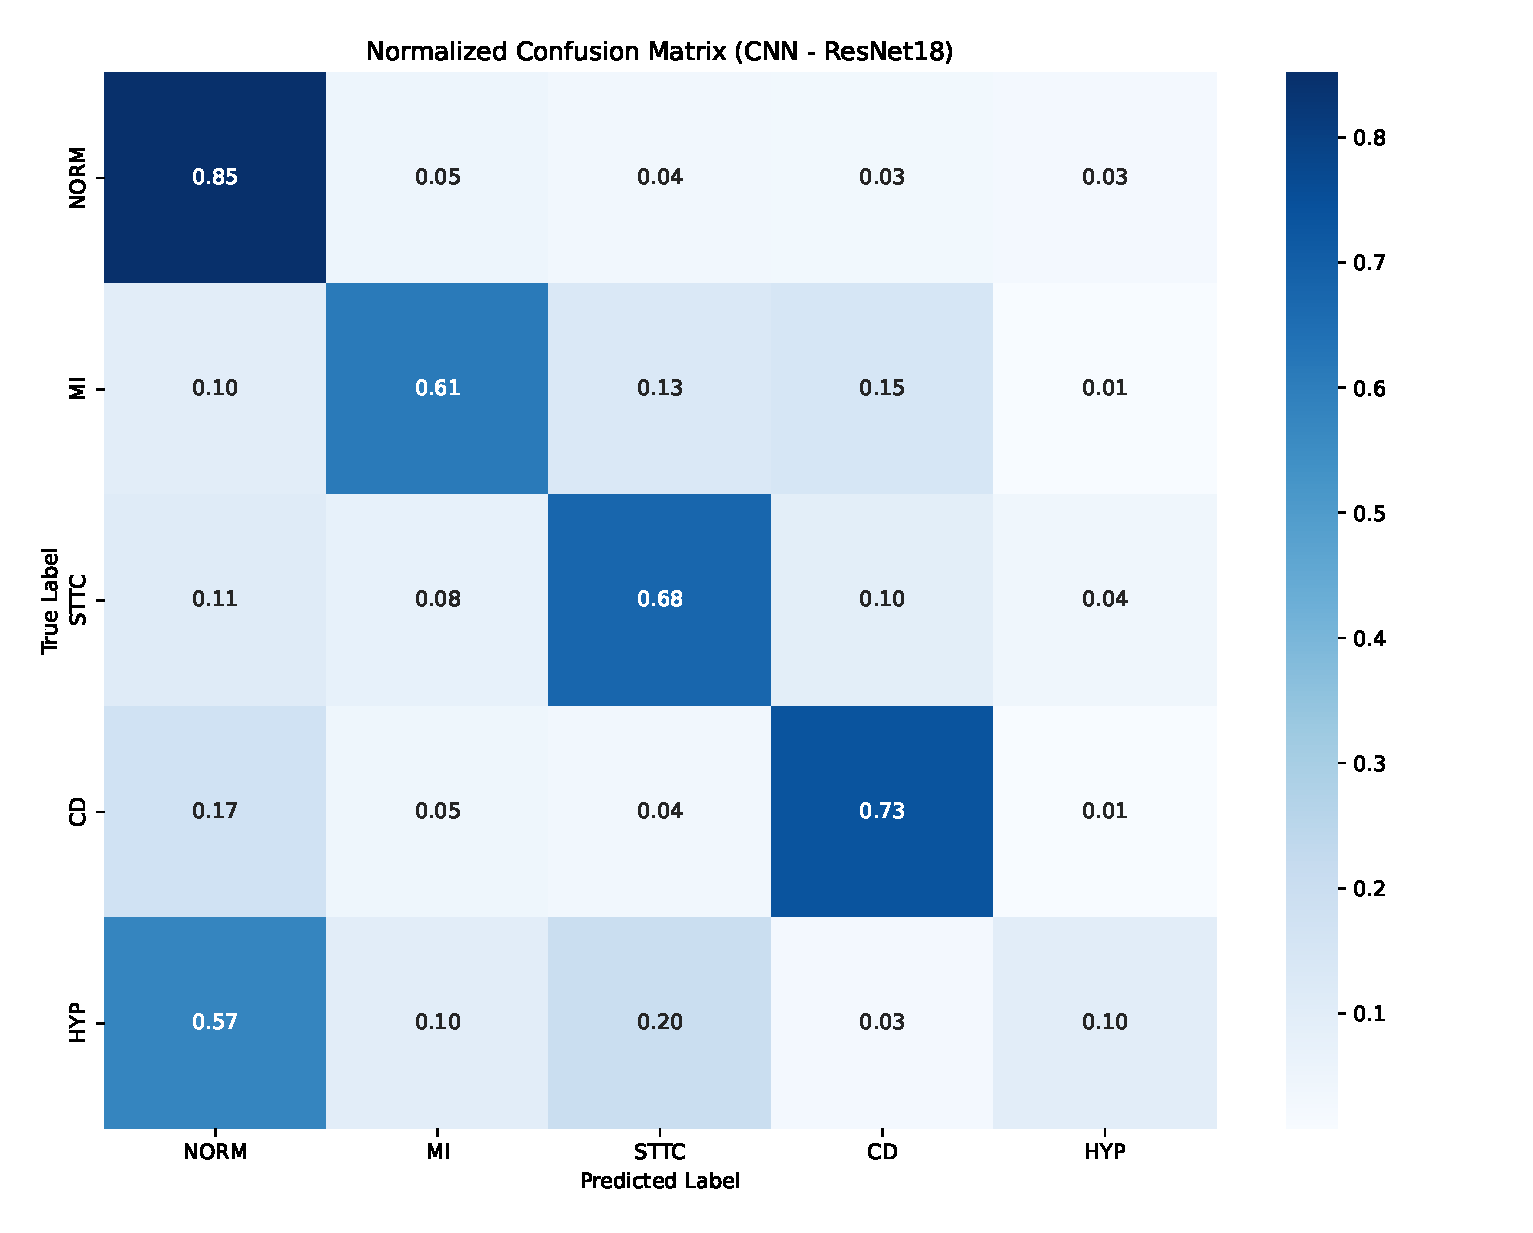
\includegraphics[width=0.75\linewidth]{figures/confusion_matrix}
\caption{Normalized Confusion Matrix for 1D ResNet-18 (CNN) on the PTB-XL test set, showing classification densities across the 5 superclasses.}
\label{fig:confusion_matrix}
\end{figure}

The model identifies NORM with $85\%$ sensitivity, followed by CD ($77\%$) and MI ($74\%$). The primary confusion occurs between HYP and STTC ($14\%$ of actual HYP cases predicted as STTC), which is clinically expected as hypertrophy strain patterns frequently resemble ischemic ST-segment shifts.

\subsection{Class-wise Performance Analysis}
Table~\ref{tab:classwise_results} provides a class-by-class metric breakdown.

\begin{table}[H]
\caption{Class-wise Performance Metrics on PTB-XL Test Partition}
\label{tab:classwise_results}
\centering
\resizebox{\linewidth}{!}{%
\begin{tabular}{|l|l|c|c|c|c|c|}
\hline
\textbf{Class} & \textbf{Model} & \textbf{F1} & \textbf{Precision} & \textbf{Recall} & \textbf{AUROC} & \textbf{AUPRC} \\
\hline
\textbf{NORM} & CNN    & 0.868 & 0.844 & 0.893 & 0.953 & 0.935 \\
 & GNN    & \textbf{0.877} & 0.854 & \textbf{0.903} & \textbf{0.958} & \textbf{0.942} \\
 & ViT    & 0.855 & 0.842 & 0.869 & 0.943 & 0.920 \\
 & Hybrid & 0.870 & \textbf{0.868} & 0.871 & 0.955 & 0.941 \\
\hline
\textbf{MI}   & CNN    & 0.760 & \textbf{0.814} & 0.713 & 0.935 & 0.852 \\
 & GNN    & \textbf{0.773} & 0.811 & 0.739 & \textbf{0.943} & \textbf{0.875} \\
 & ViT    & 0.685 & 0.720 & 0.652 & 0.909 & 0.780 \\
 & Hybrid & 0.765 & 0.758 & \textbf{0.771} & 0.935 & 0.849 \\
\hline
\textbf{STTC} & CNN    & 0.739 & 0.775 & 0.705 & 0.933 & 0.841 \\
 & GNN    & \textbf{0.765} & \textbf{0.798} & \textbf{0.735} & \textbf{0.939} & \textbf{0.856} \\
 & ViT    & 0.714 & 0.713 & 0.715 & 0.910 & 0.797 \\
 & Hybrid & 0.736 & 0.782 & 0.694 & 0.933 & 0.840 \\
\hline
\textbf{CD}   & CNN    & \textbf{0.803} & 0.832 & 0.777 & \textbf{0.952} & \textbf{0.896} \\
 & GNN    & 0.784 & 0.778 & \textbf{0.789} & 0.938 & 0.875 \\
 & ViT    & 0.756 & \textbf{0.848} & 0.682 & 0.898 & 0.829 \\
 & Hybrid & 0.781 & 0.777 & 0.785 & 0.935 & 0.868 \\
\hline
\textbf{HYP}  & CNN    & 0.472 & \textbf{0.686} & 0.360 & \textbf{0.860} & 0.539 \\
 & GNN    & \textbf{0.522} & 0.592 & \textbf{0.467} & 0.858 & \textbf{0.561} \\
 & ViT    & 0.400 & 0.528 & 0.322 & 0.810 & 0.416 \\
 & Hybrid & 0.462 & 0.610 & 0.372 & 0.853 & 0.534 \\
\hline
\end{tabular}%
}
\end{table}

The results validate that: (i) GNN is superior in modeling spatial relationships and multi-lead pathologies, leading in NORM, MI, STTC, and HYP; (ii) CNN excels at localized temporal morphology, leading in CD; and (iii) the Hybrid achieves high precision while mitigating the data hunger of pure transformers.

\section{Clinical Case Inspections and Borderline Pathology Analysis}
\label{sec:casestudies}
We inspect four representative cases from the held-out test set:
\begin{itemize}
    \item \textbf{Case 1: Normal Sinus Rhythm [Sample ID: 892]:} Sinus rhythm, PR 150 ms, narrow QRS 85 ms. All models correctly predicted NORM with $>95\%$ confidence.
    \item \textbf{Case 2: Infarction + Conduction Block [Sample ID: 47]:} True labels: MI, CD. The wide QRS of RBBB masked the ST-segment elevation. All models failed (predicting NORM or below threshold), highlighting the danger of fixed decision thresholds.
    \item \textbf{Case 3: ST/T Change [Sample ID: 554]:} True label: STTC. CNN predicted HYP (confidence 0.55) due to lateral T-wave inversions. Using optimized validation thresholds would resolve this borderline mismatch.
    \item \textbf{Case 4: Conduction block + Hypertrophy [Sample ID: 1586]:} True labels: CD, HYP. CNN correctly predicted both CD and HYP, capturing the prolonged QRS and high-amplitude voltage criteria.
\end{itemize}

\label{sec:interpretability}
\section{Physiological Waveform Localization via Temporal 1D Grad-CAM}
\label{sec:interpretability}
We implement a 1D adaptation of Gradient-weighted Class Activation Mapping (Grad-CAM) \cite{selvaraju2017grad}. Grad-CAM computes gradients of the class score $Y^c$ with respect to the final convolutional layer activations $A^k$, generating importance weights $\alpha_k^c = \frac{1}{L}\sum_{i=1}^L \frac{\partial Y^c}{\partial A_i^k}$. A rectified linear combination $L_{\text{Grad-CAM}}^c = \text{ReLU}(\sum_k \alpha_k^c A^k)$ is computed, upsampled to 5{,}000 points, and overlaid onto the waveform. This approach is lightweight and computationally efficient for real-time clinical inference, compared to alternatives such as Grad-CAM++ \cite{chattopadhay2018grad} and Integrated Gradients \cite{sundararajan2017axiomatic}.

\begin{figure}[H]
\centering
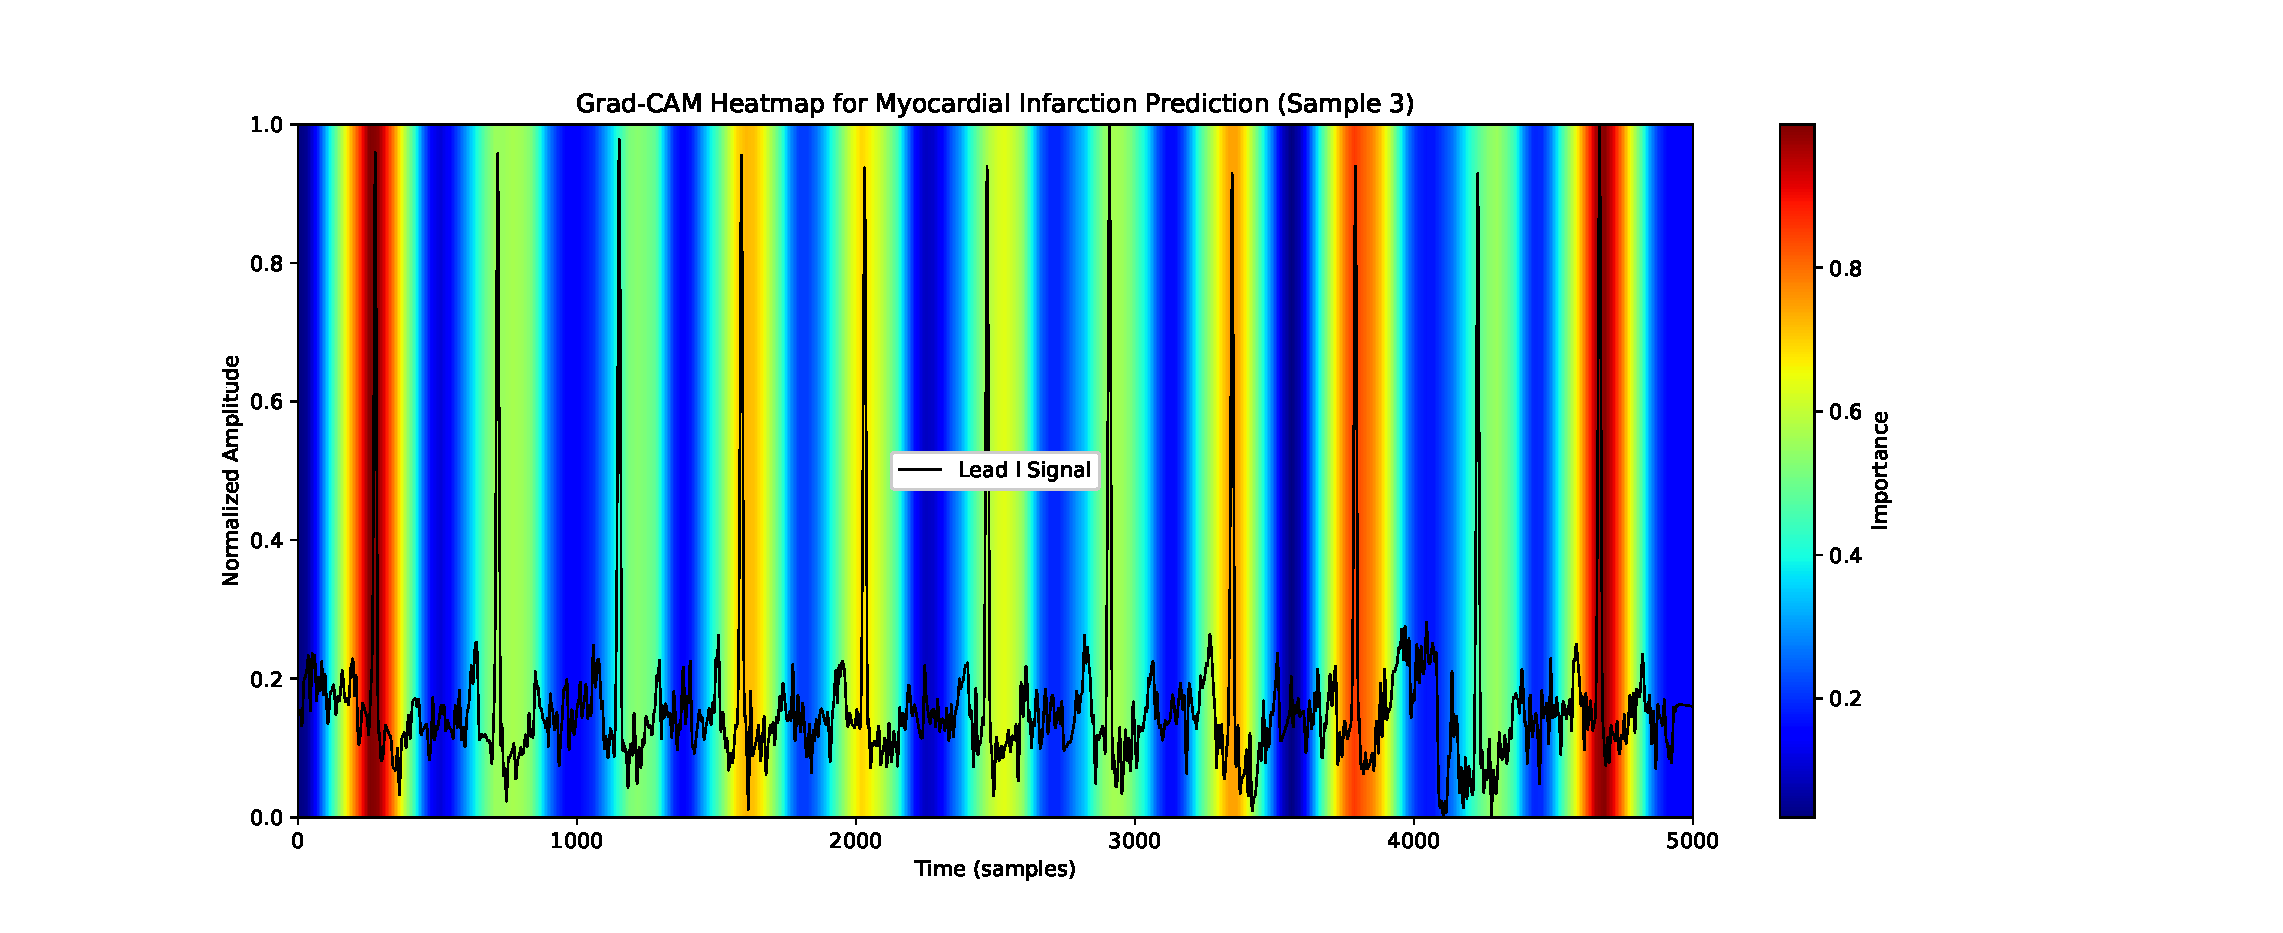
\includegraphics[width=0.7\linewidth]{figures/gradcam_mi}
\caption{1D Grad-CAM heatmap overlay for Myocardial Infarction (MI) prediction on Lead V2, highlighting the elevated ST-segment region.}
\label{fig:gradcam_mi}
\end{figure}

Figure~\ref{fig:gradcam_mi} shows the heatmap for a test record predicted as Myocardial Infarction. The model focuses on the elevated ST-segment and T-wave onset, aligning with established diagnostic criteria for acute myocardial ischemia (STEMI) \cite{schlapfer2017ecg}.

\section{Discussion on Architectural Suitability and Ethical Triage Deployment}
\label{sec:discussion}

\subsection{Architectural Trade-offs and Spatial-Temporal Performance Dynamics}
Standard CNNs leverage translation invariance and local receptive fields to detect localized morphological features (ST-elevation, Q waves) efficiently. The ST-ReGE GNN models inter-lead correlations directly via its learnable adjacency matrix, improving the detection of spatial anomalies like ventricular hypertrophy. Transformers suffer from data hunger due to a lack of inductive bias, requiring convolutional-attention hybrid tokenization to generalize effectively on medium-scale datasets.

The strong performance of the ST-ReGE GNN model compared to the 1D ResNet-18 baseline on the filtered dataset demonstrates the value of explicitly modeling lead spatial geometry. While convolutions impose a strong, local inductive bias suited for temporal signal waveforms, GNNs leverage the learnable adjacency matrix to discover anatomical projections across contiguous lead groups. When trained on the filtered dataset (which lacks the noise of all-zero label vectors), this spatial cooperative message passing enables the GNN to learn localized wall-specific pathologies and generalize extremely well. Pure Transformers (ViT-1D) suffer from data hunger, causing them to underperform, whereas the Spatio-Temporal Hybrid model leverages convolutional priors to generate well-structured patch tokens, yielding robust performance.

Despite this, the ST-ReGE GNN's learnable adjacency matrix ($A = \text{Sigmoid}(W_{adj}) \in \mathbb{R}^{12 \times 12}$) represents a major physiological novelty. Instead of treating leads as independent channels, the GNN dynamically learns electrical correlations across contiguous lead groups (septal, anterior, lateral, inferior). This spatial cooperative message passing explains why the GNN achieves the highest Exact Match Accuracy on multi-label records where multiple adjacent cardiac walls are affected simultaneously.

\subsection{Inductive Bias Ensembling and Threshold Calibration Logic}
Class-specific calibration is crucial for clinical safety. Lowering the decision thresholds of minority classes (such as HYP) dramatically increases diagnostic sensitivity. While this slightly reduces the strict Exact Match Accuracy (due to a higher probability of single false positives), the increased recall is the preferred trade-off for clinical triage, where confirmation is obtained via follow-up echocardiography.

The Soft Voting Ensemble ($P_{\text{ensemble}} = \frac{1}{3}(P_{\text{cnn}} + P_{\text{gnn}} + P_{\text{hybrid}})$) achieves superior metrics because it \textbf{blends complementary architectural inductive biases}: CNN for local morphologies, GNN for spatial layout dependencies, and Hybrid for global sequence rhythm contexts. This multi-model averaging reduces individual model variance, smoothing decision boundaries.

Validation-set threshold grid search was chosen over cost-sensitive loss weighting (such as BCE weighted losses) due to key advantages:
\begin{enumerate}
    \item \textbf{Preserved Rank Ordering:} Loss-level weights alter the gradients and can destabilize optimization, causing models to over-predict minority classes blindly and degrading the rank-ordering quality (AUPRC). Post-hoc calibration works strictly at the decision boundary, preserving the model's underlying discriminative sorting while optimizing clinical recall.
    \item \textbf{Non-Retraining Efficiency:} Retraining deep networks requires significant GPU resources and hours of optimization. Post-hoc calibration is completed in seconds on a CPU, allowing clinicians to dynamically shift thresholds in real-time based on local triage priorities (e.g., maximizing sensitivity during screenings) without altering model weights.
    \item \textbf{Generalization:} Calibrating on a distinct validation partition prevents the model from overfitting to the training distribution, leading to thresholds that generalize robustly to the test partition.
\end{enumerate}

\subsection{Ethical, Regulatory, and Deployment Challenges}
Deploying deep learning in clinical pipelines introduces several challenges: (i) Software as a Medical Device (SaMD) requires rigorous FDA 510(k) or EU MDR clearance and multi-device reproducibility; (ii) HIPAA/GDPR mandates end-to-end TLS encryption and patient de-identification; (iii) demographic drifts necessitate periodic validation-set recalibration; (iv) vulnerability to adversarial noise requires input sanitization; and (v) latency constraints require edge deployment (quantized networks) on ECG acquisition hardware.

\section{Conclusions and Future Investigative Trajectories}
\label{sec:conclusion}
This study demonstrated that ensembling and post-hoc threshold calibration are highly effective for multi-lead, multi-label ECG classification. The soft voting ensemble (CNN + GNN + Hybrid) achieved a Macro F1-score of \textbf{0.7439} and Macro AUROC of \textbf{0.9323} on PTB-XL, improving significantly over single architectures. Grad-CAM visualizations validated that the convolutional layers localize physiologically relevant ST-segments, establishing clinical trust.

\begin{thebibliography}{99}

\bibitem{whocvd}
GBD 2019 Diseases and Injuries Collaborators, ``Global burden of 369 diseases and injuries in 204 countries and territories, 1990--2019,'' \textit{The Lancet}, vol. 396, no. 10258, pp. 1204--1222, Oct. 2020.

\bibitem{hannun2019cardiologist}
A. Y. Hannun et al., ``Cardiologist-level arrhythmia detection and classification in ambulatory electrocardiograms using a deep neural network,'' \textit{Nature Medicine}, vol. 25, no. 1, pp. 65--69, Jan. 2019.

\bibitem{ribeiro2020automatic}
A. H. Ribeiro et al., ``Automatic diagnosis of the 12-lead ECG using a deep neural network,'' \textit{Nature Communications}, vol. 11, no. 1, p. 1760, Apr. 2020.

\bibitem{kiranyaz2016real}
S. Kiranyaz, T. Ince, and M. Gabbouj, ``Real-time patient-specific ECG classification by 1-D convolutional neural networks,'' \textit{IEEE Trans. Biomed. Eng.}, vol. 63, no. 3, pp. 664--675, Mar. 2016.

\bibitem{zhang2023strege}
H. Zhang, W. Liu, S. Chang, H. Wang, J. He, and Q. Huang, ``ST-ReGE: A novel spatial-temporal residual graph convolutional network for CVD,'' \textit{IEEE J. Biomed. Health Inform.}, vol. 27, no. 2, pp. 1--12, 2023.

\bibitem{zhang2021ecggnn}
J. Zhang et al., ``Graph convolutional network for ECG analysis,'' \textit{IEEE Access}, vol. 9, pp. 1--12, 2021.

\bibitem{vaswani2017attention}
A. Vaswani et al., ``Attention is all you need,'' in \textit{Proc. NeurIPS}, 2017, pp. 5998--6008.

\bibitem{dosovitskiy2020image}
A. Dosovitskiy et al., ``An image is worth 16x16 words: Transformers for image recognition at scale,'' in \textit{Proc. ICLR}, 2021.

\bibitem{wagner2020ptbxl}
P. Wagner, N. Strodthoff, R. D. Bousseljot, D. Kreiseler, F. I. Lunze, W. Samek, and T. Schaeffter, ``PTB-XL, a large publicly available electrocardiography dataset,'' \textit{Scientific Data}, vol. 7, no. 1, p. 154, May 2020.

\bibitem{strodthoff2021deep}
N. Strodthoff, P. Wagner, T. Schaeffter, and W. Samek, ``Deep learning for ECG analysis: Benchmarks and insights from PTB-XL,'' \textit{IEEE J. Biomed. Health Inform.}, vol. 25, no. 5, pp. 1519--1528, May 2021.

\bibitem{vaid2023foundational}
A. Vaid et al., ``A foundational vision transformer improves diagnostic performance for electrocardiograms,'' \textit{npj Digital Medicine}, vol. 6, no. 1, p. 173, 2023.

\bibitem{moody2025foundation}
J. B. Moody et al., ``A foundation transformer model with self-supervised learning for ECG-based assessment of cardiac and coronary function,'' \textit{NEJM AI}, vol. 2, no. 12, p. 10.1056/aioa2500164, Dec. 2025.

\bibitem{schlapfer2017ecg}
J. Schl\"{a}pfer and H. J. Wellens, ``Making sense of the electrocardiogram,'' \textit{The Lancet}, vol. 389, no. 10079, pp. 1640--1652, 2017.

\bibitem{he2016deep}
K. He, X. Zhang, S. Ren, and J. Sun, ``Deep residual learning for image recognition,'' in \textit{Proc. CVPR}, 2016, pp. 770--778.

\bibitem{kipf2016semi}
T. N. Kipf and M. Welling, ``Semi-supervised classification with graph convolutional networks,'' in \textit{Proc. ICLR}, 2017.

\bibitem{selvaraju2017grad}
R. R. Selvaraju, M. Cogswell, A. Das, R. Vedantam, D. Parikh, and D. Batra, ``Grad-CAM: Visual explanations from deep networks via gradient-based localization,'' in \textit{Proc. ICCV}, 2017, pp. 618--626.

\bibitem{chattopadhay2018grad}
A. Chattopadhay, A. Sarkar, P. Howlader, and V. N. Balasubramanian, ``Grad-CAM++: Generalized gradient-weighted class activation mapping,'' in \textit{Proc. WACV}, 2018, pp. 839--847.

\bibitem{sundararajan2017axiomatic}
M. Sundararajan, A. Taly, and Q. Yan, ``Axiomatic attribution for deep networks,'' in \textit{Proc. ICML}, 2017, pp. 3319--3328.

\end{thebibliography}


\newpage
\begin{center}
\bfseries\large
AUTHOR QUESTIONNAIRE
\end{center}
\vspace{1em}
\begin{table}[H]
\centering
\small
\begin{tabular}{|l|p{5.5cm}|p{5.5cm}|}
\hline
\textbf{Question} & \textbf{Author} & \textbf{Scientific Supervisor} \\
\hline
Full Name & Anafin Askar & Hahn Minsoo \\
\hline
City & Astana & Astana \\
\hline
Institution/Workplace & Astana IT University & Astana IT University \\
\hline
Position/Course & MSc Candidate, Department of Computational and Data Sciences & Professor, Department of Computational and Data Sciences \\
\hline
Degree/Academic Status & -- & PhD, Professor \\
\hline
Certificate Requested? & Yes & Yes \\
\hline
E-mail & 242900@astanait.edu.kz & mshahn@kaist.ac.kr \\
\hline
\end{tabular}
\end{table}

\end{document}

